
\chapter[Run-time Adaptation of System Configuration]{Run-time Adaptation of System Configuration}

\label{ch:adaptation}

%%%%%%%%%%%%%%%%%%%%%%%%%%%%%%%%%%%%%%%%%%%%%%%%%%%%%%%%%%%%%%%%%%%%%%%%%%%%%%%%%%%%%%%%%%%%%%%%%%%%%%%%%%%%%%%%%%%%%%%%%%%%%%%%%%%%%%%%%%%%%%%%
\section{Introduction}

This chapter presents an adaptation approach for reconfigurable systems.
The approach provides an efficient solution to real-time \gls{smc} methods.
We derive an adaptive \gls{smc} algorithm that adjusts its computation complexity at run time based on the quality of results.
To map our algorithm to a reconfigurable system consisting of multiple \glspl{fpga} and \glspl{cpu},
we design a pipeline-friendly data structure to make effective use of the stream computing model.
Moreover, we accelerate the algorithm with a data compression scheme and data control separation.

The key contributions of this chapter include:

\begin{itemize}
\item An adaptive \gls{smc} algorithm which adapts the size of particle set at run-time. 
The algorithm is able to reduce computation workload while maintaining the quality of results.
\item Mapping the proposed algorithm to a scalable and reconfigurable system by following the stream computing model.
A novel data structure is designed to take advantage of the architecture and to alleviate the data transfer bottleneck.
The system uses the run-time reconfigurability of \gls{fpga} to switch between computation mode and low-power mode.
\item An implementation of a robot localisation application targeting the proposed system. 
Compared to a non-adaptive and non-reconfigurable implementation, the idle power of our proposed system is reduced by 25-34\% and the overall energy consumption decreases by 17-33\%.
Our system with four \glspl{fpga} is up to 169 times faster than a single core \gls{cpu}, 41 times faster than a 1U \gls{cpu} server with 12 cores, and 3 times faster than a modelled four-\gls{gpu} system.
\end{itemize}

The rest of the chapter is organised as follows.
Section~\ref{sec:reconfig_asmc} describes the proposed adaptive \gls{smc} methods.
Section~\ref{sec:reconfig_hrs} presents the heterogeneous reconfigurable systems which is optimised for adaptive \gls{smc} methods.
Section~\ref{sec:reconfig_stream} discusses techniques which reduce the transfer overhead of particle stream.
Section~\ref{sec:reconfig_results} provides experimental results and
Section~\ref{sec:reconfig_summary} concludes our work.

%%%%%%%%%%%%%%%%%%%%%%%%%%%%%%%%%%%%%%%%
\section{Adaptive SMC Algorithm}
\label{sec:reconfig_asmc}

This section introduces an adaptive \gls{smc} algorithm which changes the number of particles at each time-step.
The algorithm is inspired by~\cite{liu07} and we transform it to a pipeline-friendly version for mapping to the reconfigurable system.
This algorithm is shown in Algorithm~\ref{algo:smc} which consists of four stages.
The basic \gls{smc} design parameters are described in Table~\ref{tab:parameters} in Chapter~\ref{ch:background}.

\begin{algorithm}
\caption{Adaptive SMC algorithm.}
{\fontsize{10}{10}\selectfont
\begin{algorithmic}[1]
\STATE{$N_{P_0} \gets N_{P_{max}}$}
\STATE{$\{s^{(i)}_0\}^{N_{P_0}}_{i=1} \gets $random set of particles}
\STATE{$t=1$}
\FOR{each step $t$}
	\STATE{$r=0$}
	\WHILE{$r \leq itl\_repeat$}
	{\color{gray} \STATE{---On \glspl{fpga}---}}
	\STATE{Sample a new state $\{s_{t+1}^{\prime(i)}\}^{N_{P_t}}_{i=1}$ from $\{s_t^{(i)}\}^{N_{P_t}}_{i=1}$} \label{algo:smc_si1}
	\STATE{Calculate unnormalised importance weights $\{w^{\prime(i)}\}^{N_{P_t}}_{i=1}$ and accumulate the weights as $w_{sum}$} \label{algo:smc_si2}
	\STATE{Calculate the lower bound of sample size $\widetilde{N_{P_{t+1}}}$ by Equation~\ref{eqt:bound2}} \label{algo:smc_lb}
	{\color{gray} \STATE{---On \glspl{cpu}---}}
	\STATE{Sort $\{s_{t+1}^{\prime(i)}\}^{N_{P_t}}_{i=1}$ in descending $\{w^{\prime(i)}\}^{N_{P_t}}_{i=1}$} \label{algo:smc_sort}
	\IF{$\widetilde{N_{P_{t+1}}} < N_{P_t}$} \label{algo:smc_rd1}
		\STATE{$N_{P_{t+1}} = max\left(\lceil\widetilde{N_{P_{t+1}}}\rceil, N_{P_t}/2\right)$}
		\STATE{Set $a = 2{N_{P_{t+1}}}-{N_{P_t}}$ and $b = {N_{P_{t+1}}}$}
		{\color{gray} \STATE{--Do the following loop in parallel--}}
		\FOR{$i$ in ${N_{P_t}}-{N_{P_{t+1}}}$} \label{algo:smc_loop1s}
			\STATE{$s_{t+1}^{\prime(i)} = \frac{s_{t+1}^{\prime(a)} w^{\prime(a)} + s_{t+1}^{\prime(b)} w^{\prime(b)}}{w^{\prime(a)} + w^{\prime(b)}}$}
			\STATE{$w^{\prime(i)} = w^{\prime(a)} + w^{\prime(b)}$}
			\STATE{$a = a+1$ and $b = b-1$}
		\ENDFOR \label{algo:smc_rd2} \label{algo:smc_loop1e}
	\ELSIF{$\widetilde{N_{P_{t+1}}} \geq {N_{P_t}}$} \label{algo:smc_rd3}
		\STATE{$a=0$ and $b=0$}
		\FOR{$i$ in ${N_{P_{t+1}}}-{N_{P_t}}$}
			\IF{$w^{\prime(a)}<w^{\prime(a+1)}$ and $a<{N_{P_{t+1}}}$}
				\STATE{$a=a+1$}
			\ENDIF
			\STATE{$s_{t+1}^{\prime({N_{P_t}}+b)} = s_{t+1}^{\prime(a)}/2$}
			\STATE{$s_{t+1}^{\prime(a)} = s_{t+1}^{\prime(a)}/2$}
			\STATE{$w^{\prime({N_{P_t}}+b)} = w^{\prime(a)}/2$}
			\STATE{$w^{\prime(a)} = w^{\prime(a)}/2$}
			\STATE{$b=b+1$}
		\ENDFOR
	\ENDIF \label{algo:smc_rd4}
	\STATE{Resample $\{s_{t+1}^{\prime(i)}\}^{{N_{P_t}}}_{i=1}$ to $\{s_{t+1}^{(i)}\}^{N_{P_{t+1}}}_{i=1}$} \label{algo:smc_r}
	\STATE{$r=r+1$}
	\ENDWHILE
\ENDFOR
\end{algorithmic}
}
\label{algo:smc}
\end{algorithm}

\paragraph{Stage 1 - Sampling and Importance Weighting (line~\ref{algo:smc_si1} to~\ref{algo:smc_si2}): }

%\subsection[Stage 1: Sampling and Importance Weighting]{Stage 1: Sampling and Importance Weighting (line~\ref{algo:smc_si1} to~\ref{algo:smc_si2})}
At the initial time-step ($t=0$), the number of particles ${N_{P_0}}$ is initialised with ${N_{P_{max}}}$ which is the maximum number of available particles.
At the subsequent time-steps, the number of particles is denoted as ${N_{P_t}}$.
Initially, the particle set $\{s_{t}^{(i)}\}^{N_{P_t}}_{i=1}$ is sampled to $\{s_{t+1}^{\prime(i)}\}^{N_{P_t}}_{i=1}$.
Then a weight from $\{w^{(i)}\}^{N_{P_t}}_{i=1}$ is assigned to each particle. 
As a result, $\{s_{t+1}^{\prime(i)}\}^{N_{P_t}}_{i=1}$ and $\{w^{(i)}\}^{N_{P_t}}_{i=1}$ give an estimation of the next state.

During sampling and importance weighting, the computation of every particle is independent of each other. 
The mapping of computation to \glspl{fpga} will be described in Section~\ref{sec:reconfig_hrs}.

\paragraph{Stage 2 - Lower Bound Calculation (line~\ref{algo:smc_lb}): }

%\subsection[Stage 2: Lower Bound Calculation]{Stage 2: Lower Bound Calculation (line~\ref{algo:smc_lb})} 
This stage derives the smallest number of particles that are needed in the next time-step in order to bound the approximation error.
The adaptive algorithm seeks a value which is less than or equal to ${N_{P_{max}}}$.
This number, denoted as $\widetilde{N_{P_{t+1}}}$, is referred to as the lower bound of sampling size.
It is calculated by Equation~\ref{eqt:bound2}:

\begin{equation}
\begin{aligned}
\widetilde{N_{P_{t+1}}} = \sigma^2 \cdot \frac{{N_{P_{max}}}}{Var(\{s_{t+1}^{\prime(i)}\}^{N_{P_t}}_{i=1})} \mbox{,}
\end{aligned}
\label{eqt:bound2}
\end{equation}

where

\begin{eqnarray}
\begin{aligned}
\sigma^2 = & \sum_{i=1}^{{N_{P_t}}}\left({w}^{(i)} \cdot s_{t+1}^{\prime(i)} \right)^2 - 2 \cdot E(\{s_{t+1}^{\prime(i)}\}^{N_{P_t}}_{i=1}) \cdot \sum_{i=1}^{N_{P_t}} \left ( ({w}^{(i)})^2 \cdot s_{t+1}^{\prime(i)} \right ) \\
& + \left(E(\{s_{t+1}^{\prime(i)}\}^{N_{P_t}}_{i=1})\right)^2 \cdot \sum_{i=1}^{N_{P_t}}({w}^{(i)})^2 \mbox{,}
\end{aligned}
\label{eqt:bound3}
\end{eqnarray}

\begin{equation}
\begin{aligned}
Var(\{s_{t+1}^{\prime(i)}\}^{N_{P_t}}_{i=1}) = \sum_{i=1}^{N_{P_t}} \left ( {w}^{(i)} \cdot (s_{t+1}^{\prime(i)})^2 \right ) - \left( E(\{s_{t+1}^{\prime(i)}\}^{N_{P_t}}_{i=1}) \right)^2 \mbox{,}
\end{aligned}
\label{eqt:bound4}
\end{equation}

\begin{equation}
\begin{aligned}
E(\{s_{t+1}^{\prime(i)}\}^{N_{P_t}}_{i=1}) = \sum_{i=1}^{N_{P_t}} {w}^{(i)} \cdot s_{t+1}^{\prime(i)} \mbox{.}
\end{aligned}
\label{eqt:bound5}
\end{equation}

As shown in Equation~\ref{eqt:bound3} to \ref{eqt:bound5}, ${w}^{(i)}$ is a normalised term. 
To calculate $w^{(i)}$, a traditional software-based approach is to iterate through the set of particles twice.
The sum of weights $w_{sum}$ and unnormalised weight $w^{\prime(i)}$ are calculated in the first iteration.
Then $w^{(i)}$ is obtained by dividing $w^{\prime(i)}$ by $w_{sum}$ in the second iteration.
However, this method is inefficient for \gls{fpga} implementation.
It is because $2 \cdot {N_{P_t}}$ cycles are needed to process ${N_{P_t}}$ pieces of data, which makes the throughput reduced to 50\%.

To fully utilise deep pipelines targeting an \gls{fpga}, we perform function transformation.
Given ${w}^{(i)} = \frac{w^{\prime(i)}}{w_{sum}}$, we move $w_{sum}$ from Equation~\ref{eqt:bound3} to \ref{eqt:bound5}.
By doing so, we obtain a transformed form as shown in Equations~\ref{eqt:bound6} to~\ref{eqt:bound8}.

\begin{eqnarray}
\begin{aligned}
\sigma^2 = & \frac{1}{(w_{sum})^2} \cdot ( \sum_{i=1}^{N_{P_t}}\left(w^{\prime(i)} \cdot s_{t+1}^{\prime(i)} \right)^2 - 2 \cdot E(\{s_{t+1}^{\prime(i)}\}^{N_{P_t}}_{i=1}) \cdot \sum_{i=1}^{N_{P_t}} \left ( (w^{\prime(i)})^2 \cdot s_{t+1}^{\prime(i)} \right )\\
& + \left(E(\{s_{t+1}^{\prime(i)}\}^{N_{P_t}}_{i=1})\right)^2 \cdot \sum_{i=1}^{N_{P_t}}(w^{\prime(i)})^2 ) \mbox{,}
\end{aligned}
\label{eqt:bound6}
\end{eqnarray}

\begin{equation}
\begin{aligned}
Var(\{s_{t+1}^{\prime(i)}\}^{N_{P_t}}_{i=1}) = \frac{1}{w_{sum}} \cdot \sum_{i=1}^{N_{P_t}} \left ( w^{\prime(i)} \cdot (s_{t+1}^{\prime(i)})^2 \right ) - \left( E(\{s_{t+1}^{\prime(i)}\}^{N_{P_t}}_{i=1}) \right)^2 \mbox{,}
\end{aligned}
\label{eqt:bound7}
\end{equation}

\begin{equation}
\begin{aligned}
E(\{s_{t+1}^{\prime(i)}\}^{N_{P_t}}_{i=1}) = \frac{1}{w_{sum}} \cdot \sum_{i=1}^{N_{P_t}} w^{\prime(i)} \cdot s_{t+1}^{\prime(i)} \mbox{.}
\end{aligned}
\label{eqt:bound8}
\end{equation}

$w_{sum}$ and $w^{\prime(i)}$ are computed simultaneously in two separate data-paths.
At the last clock cycle of the particle stream, $\sigma^2$, $Var(\{s_{t+1}^{\prime(i)}\}^{N_{P_t}}_{i=1})$ and $E(\{s_{t+1}^{\prime(i)}\}^{N_{P_t}}_{i=1})$ are obtained.
The details of the \gls{fpga} kernel design will be explained in Section~\ref{sec:reconfig_hrs}.


\paragraph{Stage 3 - Particle Set Size Tuning (line~\ref{algo:smc_sort} to~\ref{algo:smc_rd4}): }

%\subsection[Stage 3: Particle set size tuning]{Stage 3: Particle set size tuning (line~\ref{algo:smc_sort} to~\ref{algo:smc_rd4})} 
The adaptive approach tunes the particle set size to fit the lower bound ${N_{P_{t+1}}}$.
This stage is done on the \glspl{cpu} because the operations involve non-sequential data access that cannot be mapped efficiently to \glspl{fpga}.

The particles are sorted in descending order according to their weights.
As the new sample size can increase or decrease, there are two cases:

\begin{itemize}
\item {\bf Case I: Particle set reduction when $\widetilde{N_{P_{t+1}}} < {N_{P_t}}$} 

The lower bound ${N_{P_{t+1}}}$ is set to $max\left(\lceil\widetilde{N_{P_{t+1}}}\rceil, {N_{P_t}}/2\right)$.
Since the new size is smaller than the old one, some particles are combined to form a smaller particle set.
Figure~\ref{fig:tuning} illustrates the idea of particle reduction.
The first $2{N_{P_{t+1}}}-{N_{P_t}}$ particles with higher weights are kept and the remaining $2({N_{P_t}}-{N_{P_{t+1}}})$ particles are combined in pairs.
As a result, there are ${N_{P_t}}-{N_{P_{t+1}}}$ new particles injected to form the target particle set with ${N_{P_{t+1}}}$ particles.
We combine the particles deterministically to keep the statements in the loop independent of each other.
As a result, loop unrolling is undertaken to execute the statements in parallel.
The complexity of the loop is in $\bigO{\frac{{N_{P_t}}-{N_{P_{t+1}}}}{N_{parallel}}}$, where $N_{parallel}$ indicates the level of parallelism.

\setcounter{subfigure}{0}
\begin{figure}[t!]
\centering
\subfigure[Combining the last $2({N_{P_t}}-{N_{P_{t+1}}})$ particles with lower weights]{
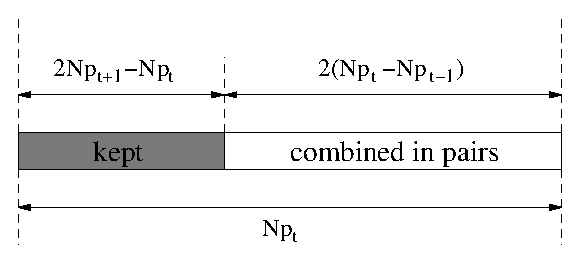
\includegraphics[width=0.45\textwidth]{4_adaptation/figures/fig_tuning1} \hfill
\label{fig:tuning1}
}
\subfigure[${N_{P_{t+1}}}$ new particles are formed]{
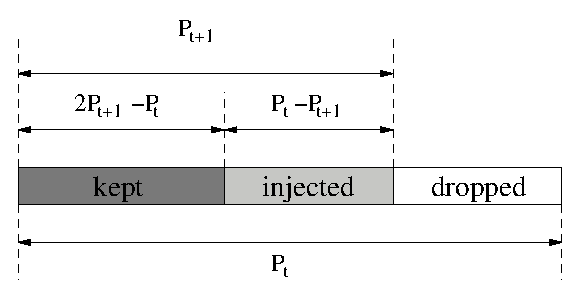
\includegraphics[width=0.45\textwidth]{4_adaptation/figures/fig_tuning2}
\label{fig:tuning2}
}
\caption{Particle set reduction.}
\label{fig:tuning}
\end{figure}

\item {\bf Case II: Particle set expansion when $\widetilde{N_{P_{t+1}}} \geq {N_{P_t}}$}

The lower bound ${N_{P_{t+1}}}$ is set to $\widetilde{N_{P_{t+1}}}$.
Some particles are taken from the original set and are inserted to form a larger set.
The particles with larger weight would have more descendants.
As shown in line~\ref{algo:smc_rd3} to~\ref{algo:smc_rd4}, the process requires picking the particle with the largest weight at each iteration of particle incision.
Since the particle set is pre-sorted, the complexity of particle set expansion is $\bigO{N_{P_{t+1}}-{N_{P_t}}}$.

\end{itemize}

\paragraph{Stage 4 - Resampling (line~\ref{algo:smc_r}): }

%\subsection[Stage 4: Resampling]{Stage 4: Resampling (line~\ref{algo:smc_r})}
Resampling is performed to pick ${N_{P_{t+1}}}$ particles from $\{s_{t+1}^{\prime(i)}\}^{N_{P_t}}_{i=1}$ to form $\{s_{t+1}^{(i)}\}^{N_{P_{t+1}}}_{i=1}$.
The process has a complexity of $\bigO{N_{P_{t+1}}}$.

%%%%%%%%%%%%%%%%%%%%%%%%%%%%%%%%%%%%%%%%
\section{Reconfigurable System Design}
\label{sec:reconfig_hrs}

This section describes the proposed heterogeneous reconfigurable system.
It is scalable to cope with different \gls{fpga} devices and applications.
The reconfigurable system also takes advantage of the run-time reconfiguration feature for power and energy reduction.

\subsection{Mapping Adaptive SMC to Reconfigurable System}
\label{sec:reconfig_arch}

The design of reconfigurable system is shown in Figure~\ref{fig:reconfig_arch}.
A heterogeneous structure is employed to make use of multiple \glspl{fpga} and \glspl{cpu}.
\glspl{fpga} and \glspl{cpu} communicate through high bandwidth buses.
\glspl{fpga} are responsible for (1) sampling, (2) importance weighting, and (3) lower bound calculation.
The data-paths on the \glspl{fpga} are fully-pipelined.
Each \gls{fpga} has its own on-board \gls{dram} to store the large amount of particle data.
On the other hand, the \glspl{cpu} gather all the particles from \glspl{fpga} to perform particle set size tuning and resampling.

Resampling requires a collective operation over the weights which makes it less readily parallelised in hardware.
Different resampling methods have been proposed aiming to parallelise the algorithm on \glspl{fpga}~\cite{bolic05} and \glspl{gpu}~\cite{murray14}.
Direct resampling methods such as stratified~\cite{sarndal03} and systematic resampling~\cite{douc05} can achieve certain degree of parallelism by removing data dependency.
Monte Carlo based methods such as Metropolis~\cite{metropolis53} and rejection sampling~\cite{neal03} strategies are more straightforward to be implemented in parallel devices.
However, Metropolis method results in a biased sample, while rejection results in non-deterministic timing.
Despite the parallelisation effort, these methods do not address the problem of non-sequential memory access pattern which has significant impact on performance when the particles are stored in off-chip memory instead of on-chip memory.

\begin{figure}[t!]
\centering
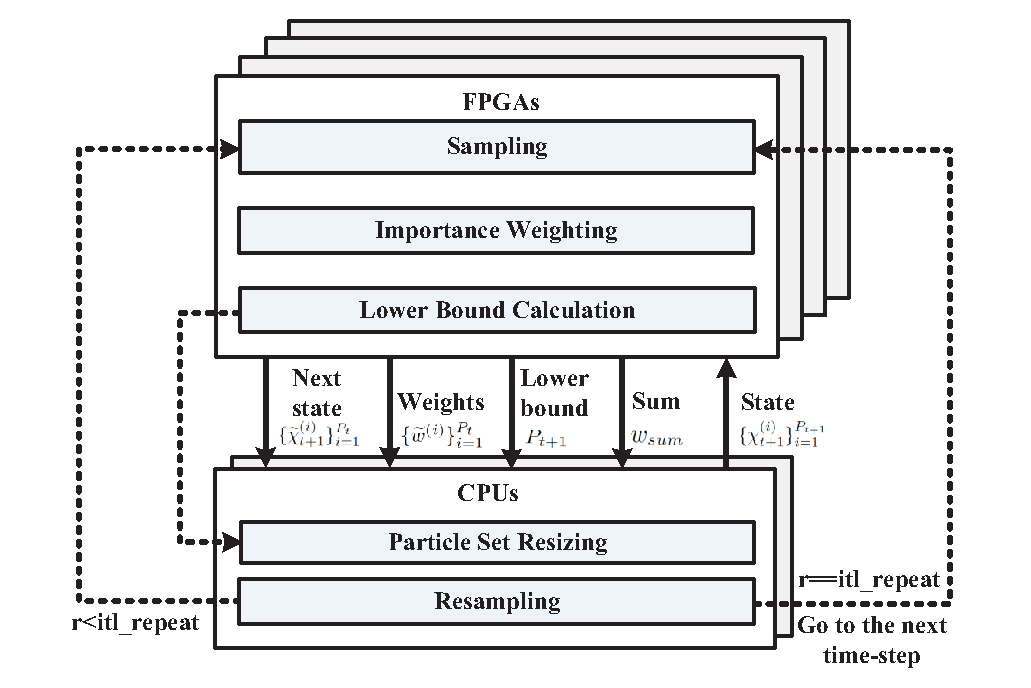
\includegraphics[width=0.8\textwidth]{4_adaptation/figures/fig_arch}
\caption[Heterogeneous reconfigurable system]{Heterogeneous reconfigurable system (Solid lines: data-paths; Dotted lines: control-paths).}
\label{fig:reconfig_arch}
\end{figure}

\begin{figure}[t!]
\centering
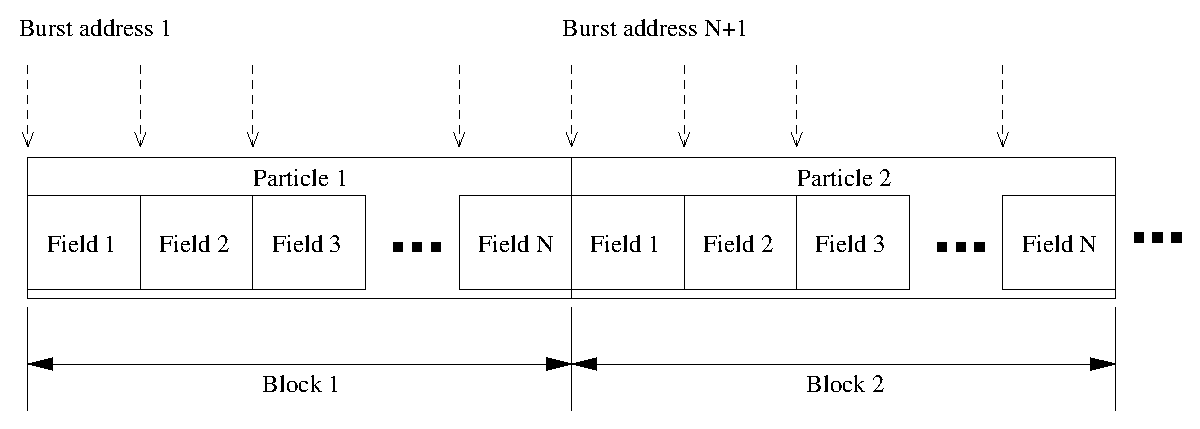
\includegraphics[width=0.8\textwidth]{4_adaptation/figures/fig_particles}
\caption{A particle stream.}
\label{fig:particles_stream}
\end{figure}

\subsection{FPGA Kernel}
Sampling, importance weighting and lower bound calculation are the most computation intensive stages.
In each time-step, these three stages are iterated for $itl\_repeat$ times.
An \gls{fpga} kernel enabling efficient acceleration is proposed.

Figure~\ref{fig:reconfig_kernel} shows the components of the \gls{fpga} kernel.
The kernel is fully pipelined to achieve one output per clock cycle.
It can also be replicated as many times as \gls{fpga} resource allow and the replications can be split across multiple \gls{fpga} boards.
The kernel takes three inputs from the \glspl{cpu} or on-board \gls{dram}: (1) states, (2) controls, and (3) seeds.
Application specific parameters are stored in ROMs.
Three building blocks corresponding to the sampling, importance weighting and lower bound calculation stages are described in Section~\ref{sec:reconfig_asmc}.

For sampling and importance weighting, the computation of each particle is independent of each other.
Particles are fed to the \glspl{fpga} as a stream shown in Figure~\ref{fig:particles_stream}.
Each block of the particle stream consists of a number of data fields which store information of a particle, where the number of data fields is application dependent.
In every clock cycle, one piece of data is transferred from the onboard memory to an \gls{fpga} data-path.
Each \gls{fpga} data-path has a long pipeline where each stage is filled with a piece of data, and therefore many particles are processed simultaneously.
Fixed-point data representation is customised at each pipeline stage to reduce the resource usage.

Meanwhile, the accumulation of $w_{sum}$ introduces a feedback loop.
A new weight comes along every cycle which is more quickly than the floating-point unit to perform addition of the previous weight.
In order to achieve one result per clock cycle, fixed-point data-path is implemented while ensuring no overflow or underflow occurs.

\begin{figure}[t!]
\centering
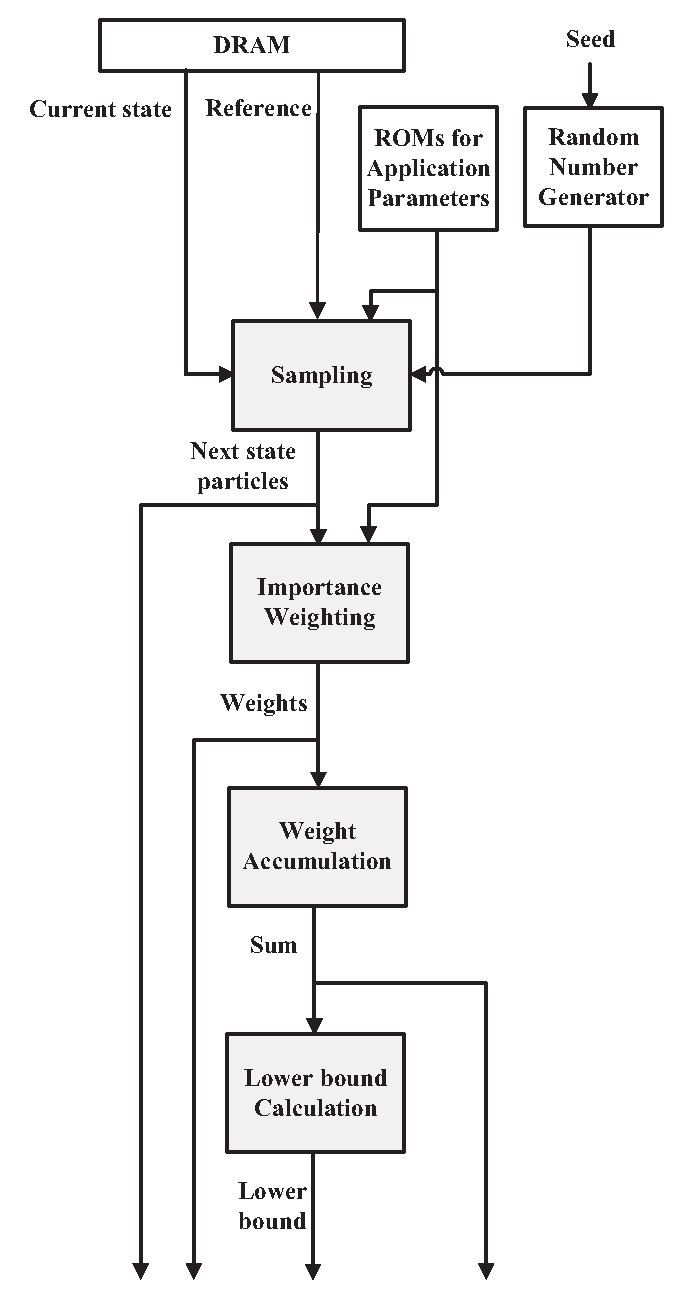
\includegraphics[width=0.5\textwidth]{4_adaptation/figures/fig_kernel}
\caption{FPGA kernel design.}
\label{fig:reconfig_kernel}
\end{figure}

\subsection{Performance Model for Run-time Reconfiguration}
\label{sec:reconfig_reconfig}

We derive a model to analyse the computation time of reconfigurable system.
The model helps us to design a configuration schedule that satisfies the real-time requirement and, if necessary, amend the application's specification.
The model will be validated by experiments in Section~\ref{sec:reconfig_results}.

The computation time, $T_{comp}$, of reconfigurable system consists of three components: (1) Data-path time $T_{datapath}$, (2) \gls{cpu} time $T_{cpu}$, and (3) Data transfer time $T_{tran}$ as shown in Equation~\ref{eqt:total}:

\begin{equation}
\begin{aligned}
T_{comp} = itl\_repeat \cdot \left ( T_{datapath} + T_{cpu} + T_{tran} \right ) \mbox{,}
\end{aligned}
\label{eqt:total}
\end{equation}

where $itl\_repeat$ represents the number of times that the sampling, importance weighting and resampling processes are repeated in every time-step.

\textbf{Data-path time}, $T_{datapath}$, denotes the time spent on the \glspl{fpga}.

\begin{equation}
\begin{aligned}
T_{datapath} = \left(\frac{{N_{P_t}}}{freq_{fpga} \cdot N_{datapath}} + L - 1 \right) \frac{1}{N_{fpga}} \mbox{,}
\end{aligned}
\label{eqt:kernel}
\end{equation}

where $P_t$ denotes the number of particles at the current time-step and $freq_{fpga}$ denotes the clock frequency of the \glspl{fpga}.
$L$ is the length of the pipeline.
$N_{datapath}$ denotes the number of data-paths on one \gls{fpga} board.
$N_{fpga}$ is the number of \gls{fpga} boards in the system.

\textbf{\gls{cpu} time}, $T_{cpu}$, denotes the time spent on the \glspl{cpu}.

\begin{equation}
\begin{aligned}
T_{cpu} = \alpha \cdot \frac{{N_{P_t}}}{freq_{cpu}} \cdot \left(1-par+\frac{par}{N_{thread}}\right) \mbox{,}
\end{aligned}
\label{eqt:host}
\end{equation}

where the clock frequency and number of threads of the \glspl{cpu} are represented by $freq_{cpu}$ and $N_{thread}$ respectively.
$par$ is an application-specific parameter in the range of $[0,1]$ which represents the ratio of \gls{cpu} instructions that are parallelisable, and $\alpha$ is a scaling constant derived empirically.

\textbf{Data transfer time}, $T_{tran}$, denotes the time of moving a particle stream between the \glspl{fpga} and the \glspl{cpu}.

\begin{equation}
\begin{aligned}
T_{tran} = \frac{(2 \cdot df + 1) \cdot W_{data} \cdot {N_{P_t}}}{freq_{bus} \cdot lane \cdot eff \cdot N_{fpga}} \mbox{,}
\end{aligned}
\label{eqt:data}
\end{equation}

where $df$ is the number of data fields of a particle.
For example, if a particle contains the information of coordinates ($x$, $y$) and heading $h$, $df=3$.
Given that the constant 1 represents the weight and the constant 2 accounts for the movement of data in and out of the \glspl{fpga},
and $W_{data}$ is the bit-width of one data field, the expression $(2 \cdot df + 1) \cdot W_{data}$ is regarded as the size of a particle.
$freq_{bus}$ is the clock frequency of the bus connecting the \glspl{cpu} to \glspl{fpga} and $lane$ is the number of bus lanes connected to one \gls{fpga}.
Since many buses, such as the PCI Express Bus, encode data during transfer, the effective data are denoted by $eff$ (in PCI Express Gen2 the value is 8/10).
In our previous work~\cite{chau13arc}, the data transfer time has a significant performance impact on reconfigurable system.
To reduced the data transfer overhead, we introduce a data compression technique that will be described in Section~\ref{sec:reconfig_stream}.

In real-time applications, each time-step is fixed and is known as the real-time bound $T_{rt}$.
The derived model helps system designers to ensure that the computation time $T_{comp}$ is shorter than $T_{rt}$.
An idle time $T_{idle}$ is introduced to represent the time gap between the computation time and real-time bound.
It is calculated by Equation~\ref{eqt:idle}:

\begin{equation}
\begin{aligned}
T_{idle} = T_{rt} - T_{comp} \mbox{.}
\end{aligned}
\label{eqt:idle}
\end{equation}

Figure~\ref{fig:timing1} illustrates the power consumption of a reconfigurable system without run-time reconfiguration.
It shows that the \glspl{fpga} are still drawing power after the computation finishes.
By exploiting run-time reconfiguration as shown in Figure~\ref{fig:timing2}, the \glspl{fpga} are loaded with a low-power configuration during the idle period.
Such configuration minimises the amount of active resources and clock frequency.
Equation~\ref{eqt:sleep} describes the sleep time when the \glspl{fpga} are idle and being loaded with the low-power configuration.
If the sleep time is positive, reconfiguration would be helpful in these situations, where the sleep time is expressed as:

\begin{equation}
\begin{aligned}
T_{sleep} = T_{idle} - T_{config} \mbox{.}
\end{aligned}
\label{eqt:sleep}
\end{equation}

\textbf{Configuration time}, $T_{config}$, denotes the time needed to download a configuration bit-stream to the \glspl{fpga}:

\begin{equation}
\begin{aligned}
T_{config} = \frac{size_{bs}}{freq_{config} \cdot W_{config}} \mbox{,}
\end{aligned}
\label{eqt:cf}
\end{equation}

where $size_{bs}$ represents the size of bitstream in bits, and $freq_{config}$ is the configuration clock frequency in Hz and $W_{config}$ is the bit-width of the configuration port.

\setcounter{subfigure}{0}
\begin{figure}[t!]
\centering
\subfigure[Without reconfiguration]{
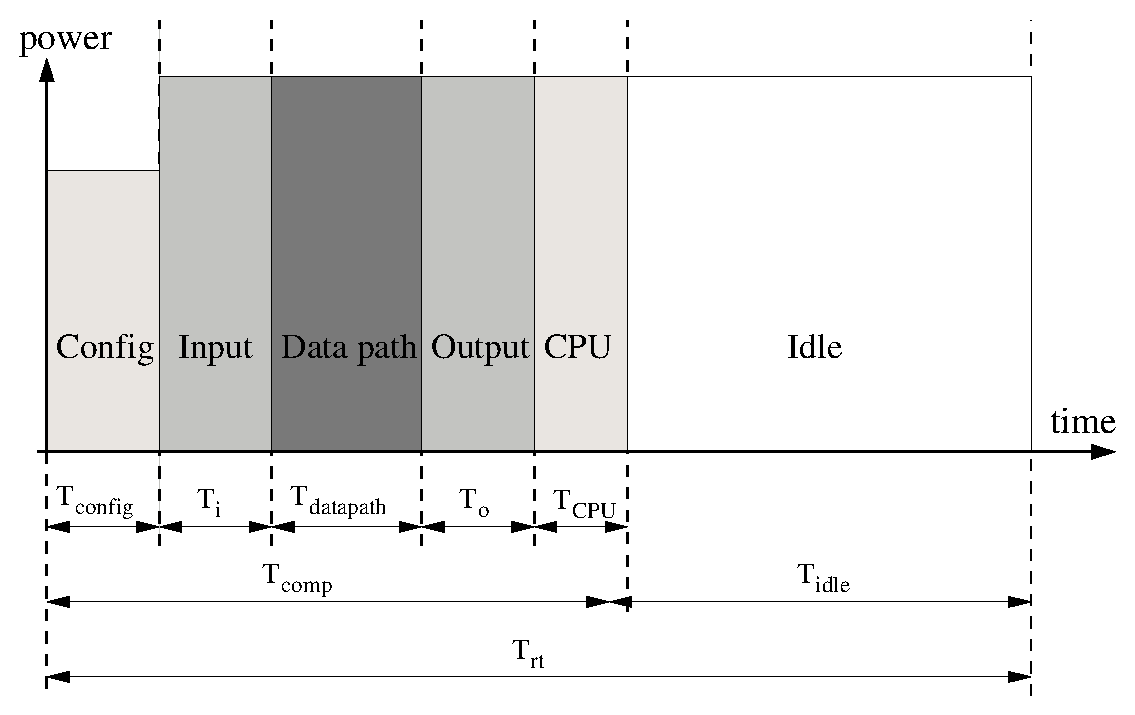
\includegraphics[width=0.6\textwidth]{4_adaptation/figures/fig_timing1} \hfill
\label{fig:timing1}
}
\subfigure[With reconfiguration to low-power mode during idle]{
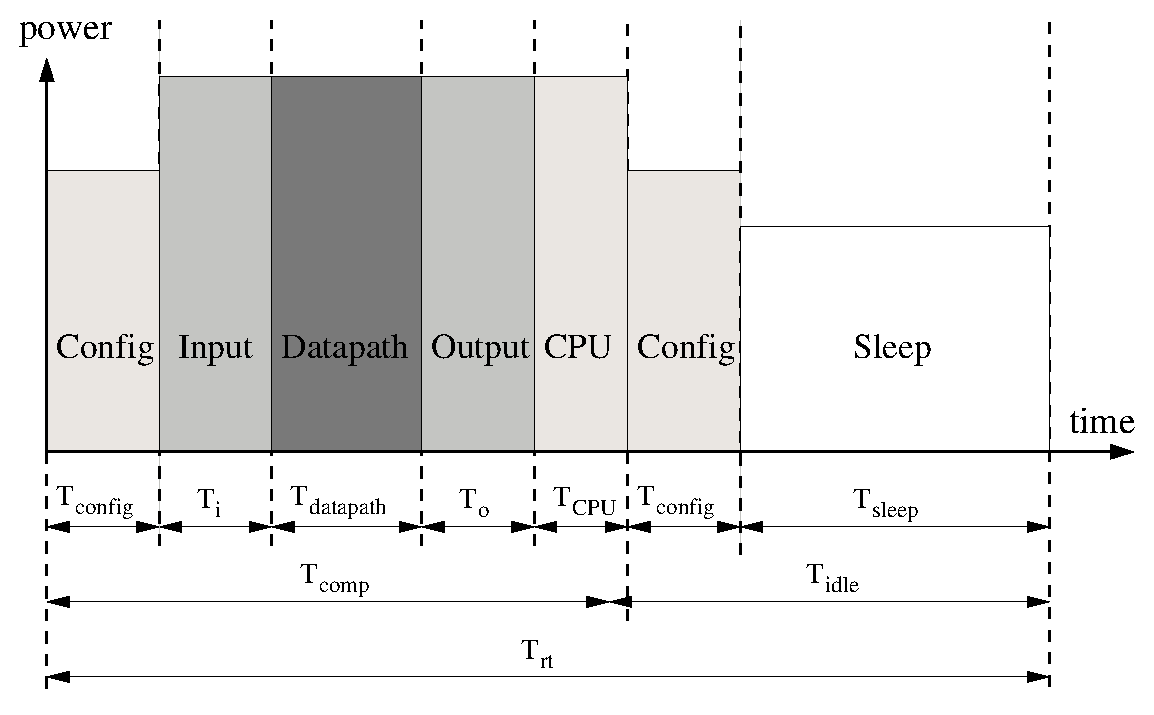
\includegraphics[width=0.6\textwidth]{4_adaptation/figures/fig_timing2}
\label{fig:timing2}
}
\caption{Power consumption of the reconfigurable system over time.}
\label{fig:timing}
\end{figure}

%%%%%%%%%%%%%%%%%%%%%%%%%%%%%%%%%%%%%%%%
\section{Optimising Transfer of Particle Stream}
\label{sec:reconfig_stream}

In Section~\ref{sec:reconfig_hrs}, the data transfer time depends on the number of particles and the bus bandwidth between the \glspl{cpu} and \glspl{fpga}.
It can be a major performance bottleneck as depicted in~\cite{chau13arc}.
Refer to Figure~\ref{fig:particles_resampling_unopt}, each block stores the data of a particle.
When the \glspl{cpu} finish processing, all data are transferred from the \glspl{cpu} to the \glspl{fpga}.
The data transfer time cannot be reduced by either implementing more \gls{fpga} data-paths or increasing the \glspl{fpga}' clock frequency because the bottleneck is at the bus connecting the \glspl{cpu} and \glspl{fpga}.

To improve the data transfer performance, we design a data structure which facilitates compression of particles.
The idea comes from an observation of the resampling process - some particles are eliminated and the vacancies are filled by replicating non-eliminated particles.
Replication means data redundancy exists.
For example, in the original data structure shown in Figure~\ref{fig:particles_resampling_unopt}, 
particle~1 has three replicates and particle~2 is eliminated, therefore, particle~1 is stored and transferred for three times.

By using the data structure in Figure~\ref{fig:particles_resampling_opt}, data redundancy is eliminated by storing every particle once.
Each particle is also transferred once.
As a result, the data transfer time and memory space are reduced.

\setcounter{subfigure}{0}
\begin{figure}[t!]
\centering
\subfigure[Particle stream before compression]{
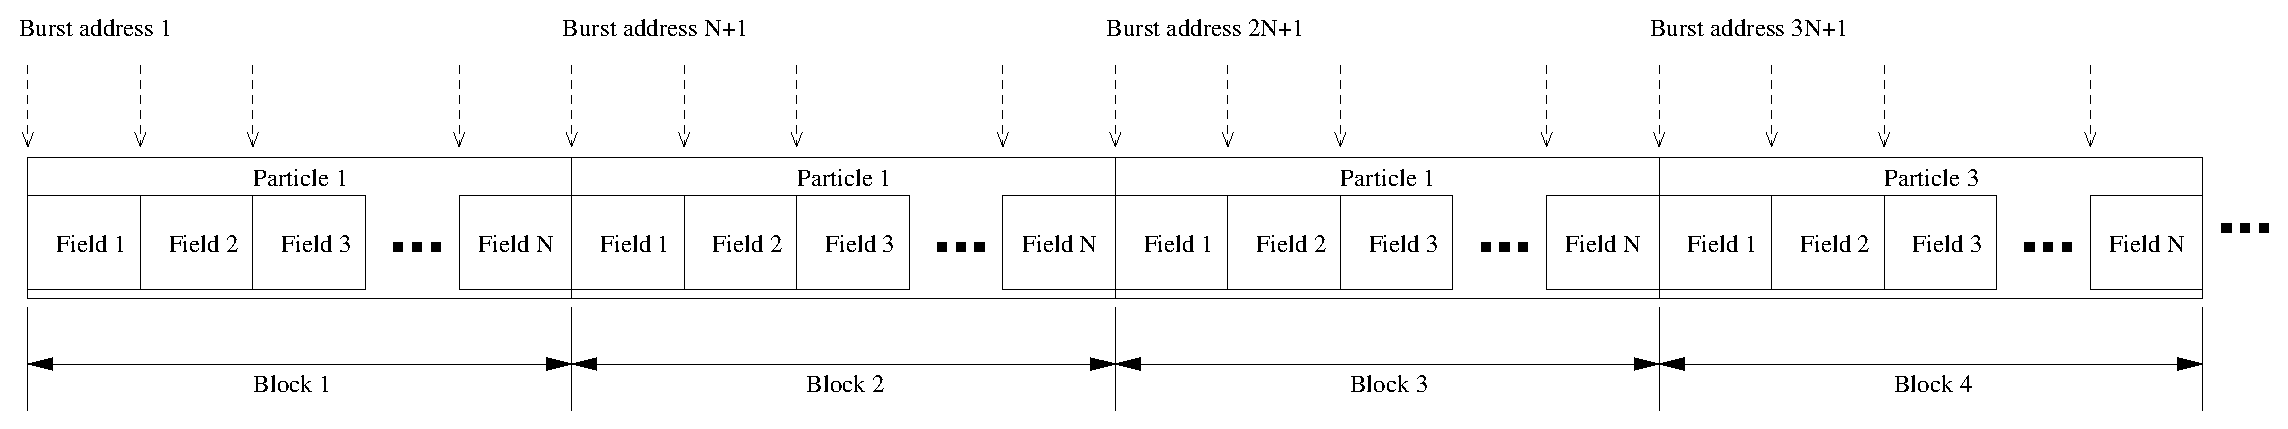
\includegraphics[width=\textwidth]{4_adaptation/figures/fig_particles_resampling}
\label{fig:particles_resampling_unopt}
}
\subfigure[Compressed particle stream]{
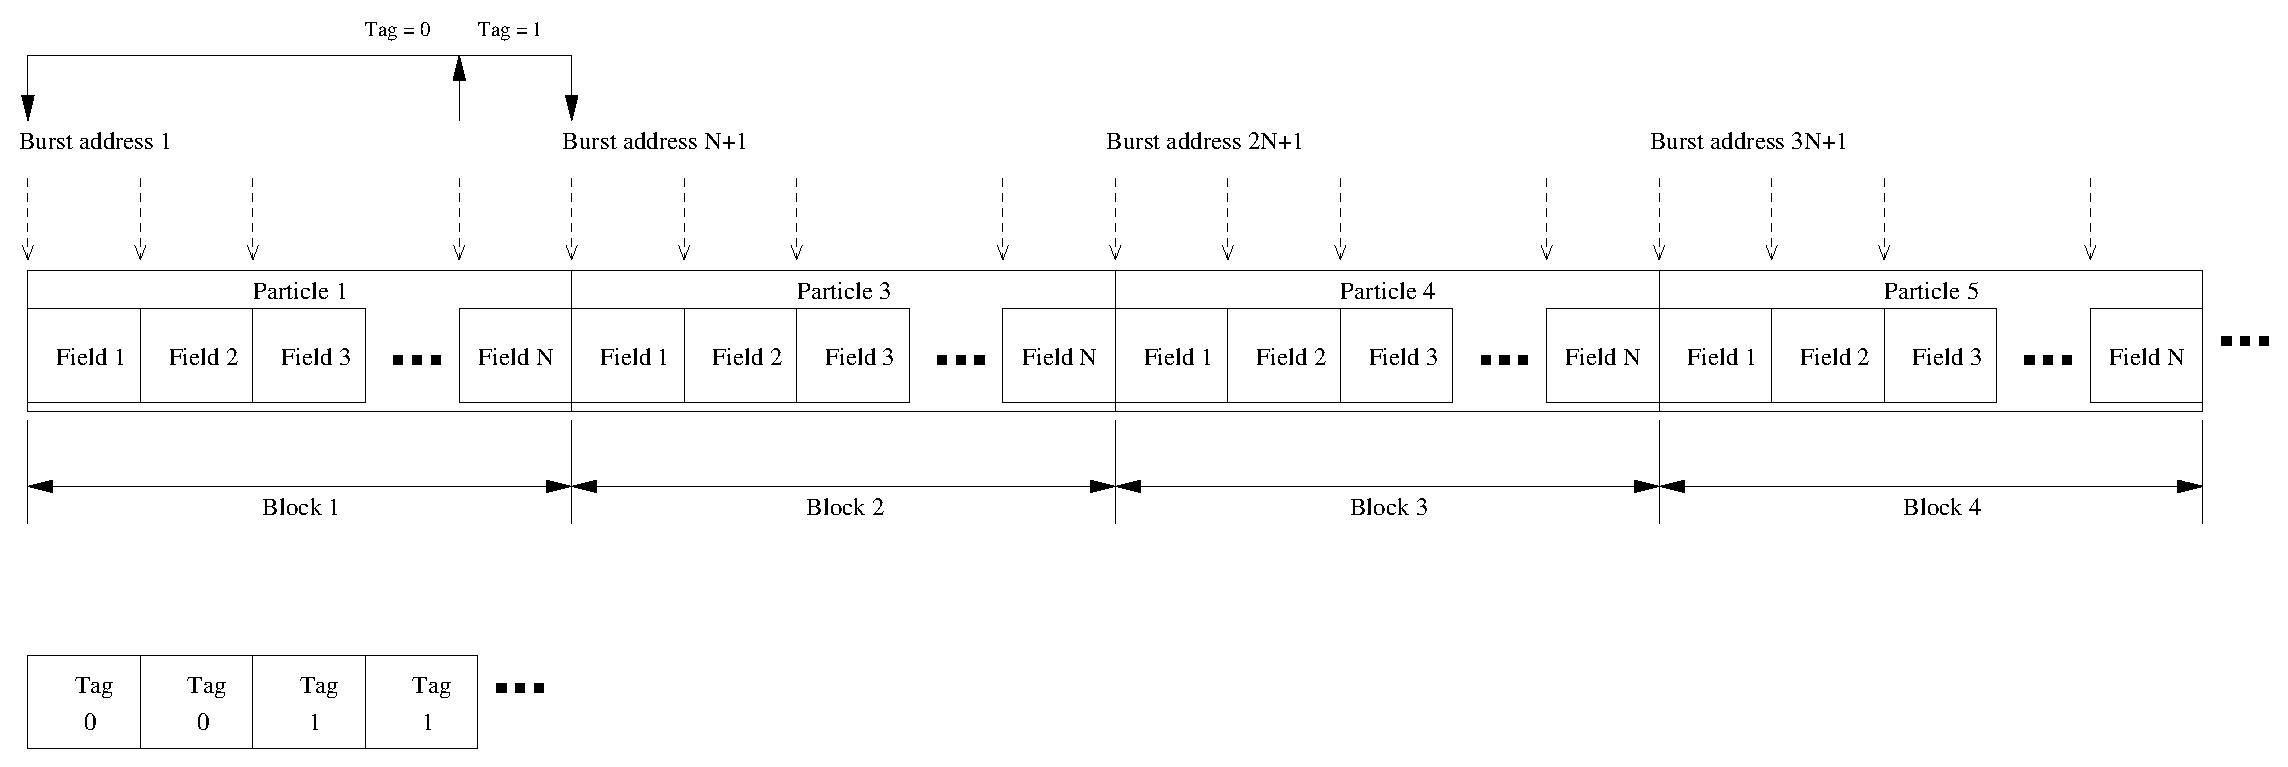
\includegraphics[width=\textwidth]{4_adaptation/figures/fig_particles_resampling_b}
\label{fig:particles_resampling_opt}
}
\caption{Compressing particle stream: After the resampling process, some particles are eliminated and the remaining particles are replicated. Data compression is applied so that every particle is stored and transferred once only.}
\label{fig:particles_resampling}
\end{figure}

A reconfigurable system often contains \gls{dram} which transfers data in burst in order to maximise the memory bandwidth.
This works fine with the original data structure where the data are organised as a sequence from the lower address space to the upper.
However, using the new data structure, the data access pattern is not sequential any more, the address goes back and forth.
The \gls{dram} controller needs to be modified so that the transfer throughput would not be affected by the change of data access pattern.
As illustrated in Figure~\ref{fig:particles_resampling_opt}, a tag sequence is used to indicate the address of the next block.
For example, after reading the data of particle~1, the burst address is at $N$.
If the tag is one, the next burst address will point to the address of the next block at $N+1$.
Otherwise, the burst address will point to the start address of the current block (which is $1$).
The data are still addressed in burst so the performance is not degraded.

The data transfer time with compression, $T_{Tran}$, is shown below:

\begin{equation}
\begin{aligned}
T_{tran} = \frac{(\frac{df}{Rep} + df + 1) \cdot W_{data} \cdot {N_{P_t}}}{freq_{bus} \cdot lane \cdot eff \cdot N_{fpga}} \mbox{,}
\end{aligned}
\label{eqt:data_opt}
\end{equation}

where $Rep$ is the average number of replication of the particles,
and therefore the size of the resampled particle stream is reduced by a ratio of $Rep$ when compared to that without compression.
The range of $Rep$ is from 1 to $N_{P_t}$, depending on the distribution of particles after the resampling process.
The effect of $Rep$ on data transfer time will be evaluated in the next section.

%%%%%%%%%%%%%%%%%%%%%%%%%%%%%%%%%%%%%%%%
\section{Experimental Results}
\label{sec:reconfig_results}

To evaluate the performance of the reconfigurable system and make comparison with the other systems, 
we implement an application which uses \gls{smc} for localisation and tracking of mobile robot.
The application is proposed in~\cite{montemerlo02} to track location of moving objects conditioned upon robot poses over time.
Given a priori learned map, a robot receives sensor values and moves at regular time intervals. 
Meanwhile, $M$ moving objects are tracked by the robot.
The states of the robot and objects at time $t$ are represented by a state vector $X_t$:
 
\begin{equation}
\begin{aligned}
X_t = \{R_t, H_{t,1}, H_{t,2}, ..., H_{t,M}\} \mbox{.}
\end{aligned}
\end{equation}

$R_t$ denotes the robot's pose at time $t$, and $H_{t,1}, H_{t,2}, ..., H_{t,M}$ denote the locations of the $M$ objects at the same time.

The following equation is used to represent the posterior of the robot's location:

\begin{equation}
\begin{aligned}
p(X_t|Y_t,U_t) = p(R_t|Y_t,U_t) \prod_{m=1}^M p(H_{t,m}|R_t,Y_t,U_t) \mbox{,}
\end{aligned}
\end{equation}

where $Y_t$ is the sensor measurement and $U_t$ is the control of the robot at time $t$.
The robot path posterior $p(R_t|Y_t,U_t)$ is represented by a set of robot-particles.
The distribution of an object's location $p(H_{t,m}|R_t,Y_t,U_t)$ is represented by a set of object-particles, where each object-particle set is attached to one particular robot-particle.
In other words, if there are ${N_{P_r}}$ robot-particles representing the posterior over robot path, there are ${N_{P_r}}$ object-particle sets, each has ${N_{P_h}}$ particles.

In the application, the area of the map is 12m by 18m.
The robot makes a movement of 0.5m every five seconds, i.e. $T_{rt} = 5$.
The robot can track eight moving objects at the same time.
A maximum of 8192 particles are used for robot-tracking and each robot-particle is associated with 1024 object-particles.
Therefore, the maximum number of data-path cycles is $8 \times 8192 \times 1024=67,108,864$.
Each particle being streamed into the \glspl{fpga} contains coordinates ($x$,$y$) and heading $h$ which are represented by three single precision floating-point numbers.
For the particle being streamed out of the \glspl{fpga}, it also contains a weight in addition to the coordinates.
From Equation~\ref{eqt:data}, the size of a particle is $(2 \cdot 3 + 1) \cdot 32 \mbox{ bits} = 224 \mbox{ bits}$.

\subsection{System Settings}

\textbf{Reconfigurable system}: Two reconfigurable systems from Maxeler Technologies are used.
The system is developed using MaxCompiler, which adopts a stream computing model.
\begin{itemize}
\item \textit{MaxWorkstation} is a microATX form factor system which is equipped with one Xilinx Virtex-6 XC6VSX475T \gls{fpga}.
The \gls{fpga} has 297,600 \glspl{lut}, 595,200 registers, 2,016 \glspl{dsp} and 1,064 block \glspl{ram}. 
The \gls{fpga} board is connected to an Intel i7-870 \gls{cpu} (4 physical cores, 8 threads in total, clocked at 2.93 GHz) via a PCI Express Gen2 x8 bus.
The maximum bandwidth of the PCI Express bus is 2 GB/s according to the specification provided by Maxeler Technologies.
\item \textit{MPC-C500} is a 1U server accommodating four \gls{fpga} boards, each of which has a Xilinx Virtex-6 XC6VSX475T \gls{fpga}.
Each \gls{fpga} board is connected to two Intel Xeon X5650 \glspl{cpu} (12 physical cores, 24 threads in total, clocked at 2.66 GHz) via a PCI Express Gen2 x8 bus.
\end{itemize}

To support run-time reconfigurability, two \gls{fpga} configurations are used:
\begin{itemize}
\item {\it Sampling and importance weighting configuration} is clocked at 100 MHz.
Two data-paths are implemented on one \gls{fpga} to process particles in parallel.
The total resource usage is 231,922 \glspl{lut} (78\%), 338,376 registers (56\%), 1,934 \glspl{dsp} (96\%) and 514 block \glspl{ram} (48\%).
\item {\it Low-power configuration} is clocked at 10 MHz, with 5,962 \glspl{lut} (2\%), 6,943 registers (1\%) and 12 block \glspl{ram} (1\%).
It uses minimal resources just to maintain communication between the \glspl{fpga} and \glspl{cpu}.
\end{itemize}

\textbf{\gls{cpu}}: The \gls{cpu} performance results are obtained from a 1U server that hosts two Intel Xeon X5650 \glspl{cpu}. 
Each \gls{cpu} is clocked at 2.66 GHz.
The program is written in C language and optimised by Intel Compiler with SSE4.2 and flag {\it -fast} enabled.
OpenMP is used to utilise all the processor cores.

\textbf{\gls{gpu}}: An NVIDIA Tesla C2070 \gls{gpu} is hosted inside a 4U server.
It has 448 cores running at 1.15 GHz and has a peak performance by 1288 GFlops.
The program is written in C for CUDA and optimised to use all the cores available.
To get more comprehensive results for comparison, we also estimate the performance of multiple \gls{gpu}s.
The estimation is based on the fact that the first three stages (sampling, importance weighting, lower bound calculation) can be evenly distributed to every \gls{gpu} and be computed independently, 
so the data-path and data transfer speedup scales linearly with the number of \gls{gpu}s.
On the other hand, the last two stages (particle set resizing, resampling) are computed on the \gls{cpu} no matter how many \gls{gpu}s are used.
Therefore, the \gls{cpu} time does not scale with the number of \gls{gpu}s.

\subsection{Adaptive SMC versus Non-adaptive SMC}
The comparison of adaptive and non-adaptive \gls{smc} is shown in Table~\ref{tab:smc}.
Both model estimation and experimental results are listed.
Initially, the maximum number of particles are instantiated for global localisation.

For the non-adaptive scheme, the particle set size does not change.
The total computation time estimated and measured are 1.328 seconds and 1.885 seconds, respectively.
The measured computation time is longer due to the difference between the effective and maximum bandwidth of the PCI Express bus.

\begin{table}[ht]
	\centering
	\setlength{\tabcolsep}{5pt}
	\begin{spacing}{1.0}
	\caption[Comparison of adaptive and non-adaptive SMC on reconfigurable system.]{Comparison of adaptive and non-adaptive SMC on reconfigurable system (MaxWorkstation with one FPGA, no data compression is applied).}
	\label{tab:smc}{
	\smallskip
		\begin{tabular}{l || c c | c c}
			\hline
			 \multirow{2}{*}{}  & \multicolumn{2}{c|}{Non-adaptive \gls{smc}} & \multicolumn{2}{c}{Adaptive \gls{smc}} \\
			\hline
			  & Model & Experiment & Model & Experiment \\
			\hline
			\hline
			 Number of particles & \multicolumn{2}{c|}{67M} & \multicolumn{2}{c}{573k} \\
			\hline
			 Data-path time $T_{datapath}$ (s) 		& 0.336 & 0.336 & 0.003 & 0.003 \\
			 \gls{cpu} time $T_{cpu}$ (s) 				& 0.117 & 0.117 & 0.001 & 0.001 \\
			 Data time $T_{tran}$ (s) 				& 0.875 & 1.432 & 0.007 & 0.012 \\
			 Total computation time $T_{comp}$ (s)			& 1.328 & 1.885 & 0.011	& 0.016 \\
			\hline
			 Comp. speedup (higher is better)		& 1x	& 1x	& 120.7x	& 117.8x \\
			\hline
		\end{tabular}
	}
	\end{spacing}
\end{table}

For the adaptive scheme, the number of particles varies from 573k to 67M, and the computation time scales linearly with the number of particles.
From Table~\ref{tab:smc}, both the model and experiment show 99\% reduction in computation time.

Figure~\ref{fig:adaptive} shows how both the number of particles and the components of total computation time vary over the wall-clock time (passage of time from the start to the completion of the application).
Although the number of particles is reduced in the proposed design, the results in Figure~\ref{fig:error} show that the localisation error is not adversely affected.
The error is the highest during initial global localisation and it is reduced when the robot moves.

\begin{figure}[t!]
\centering
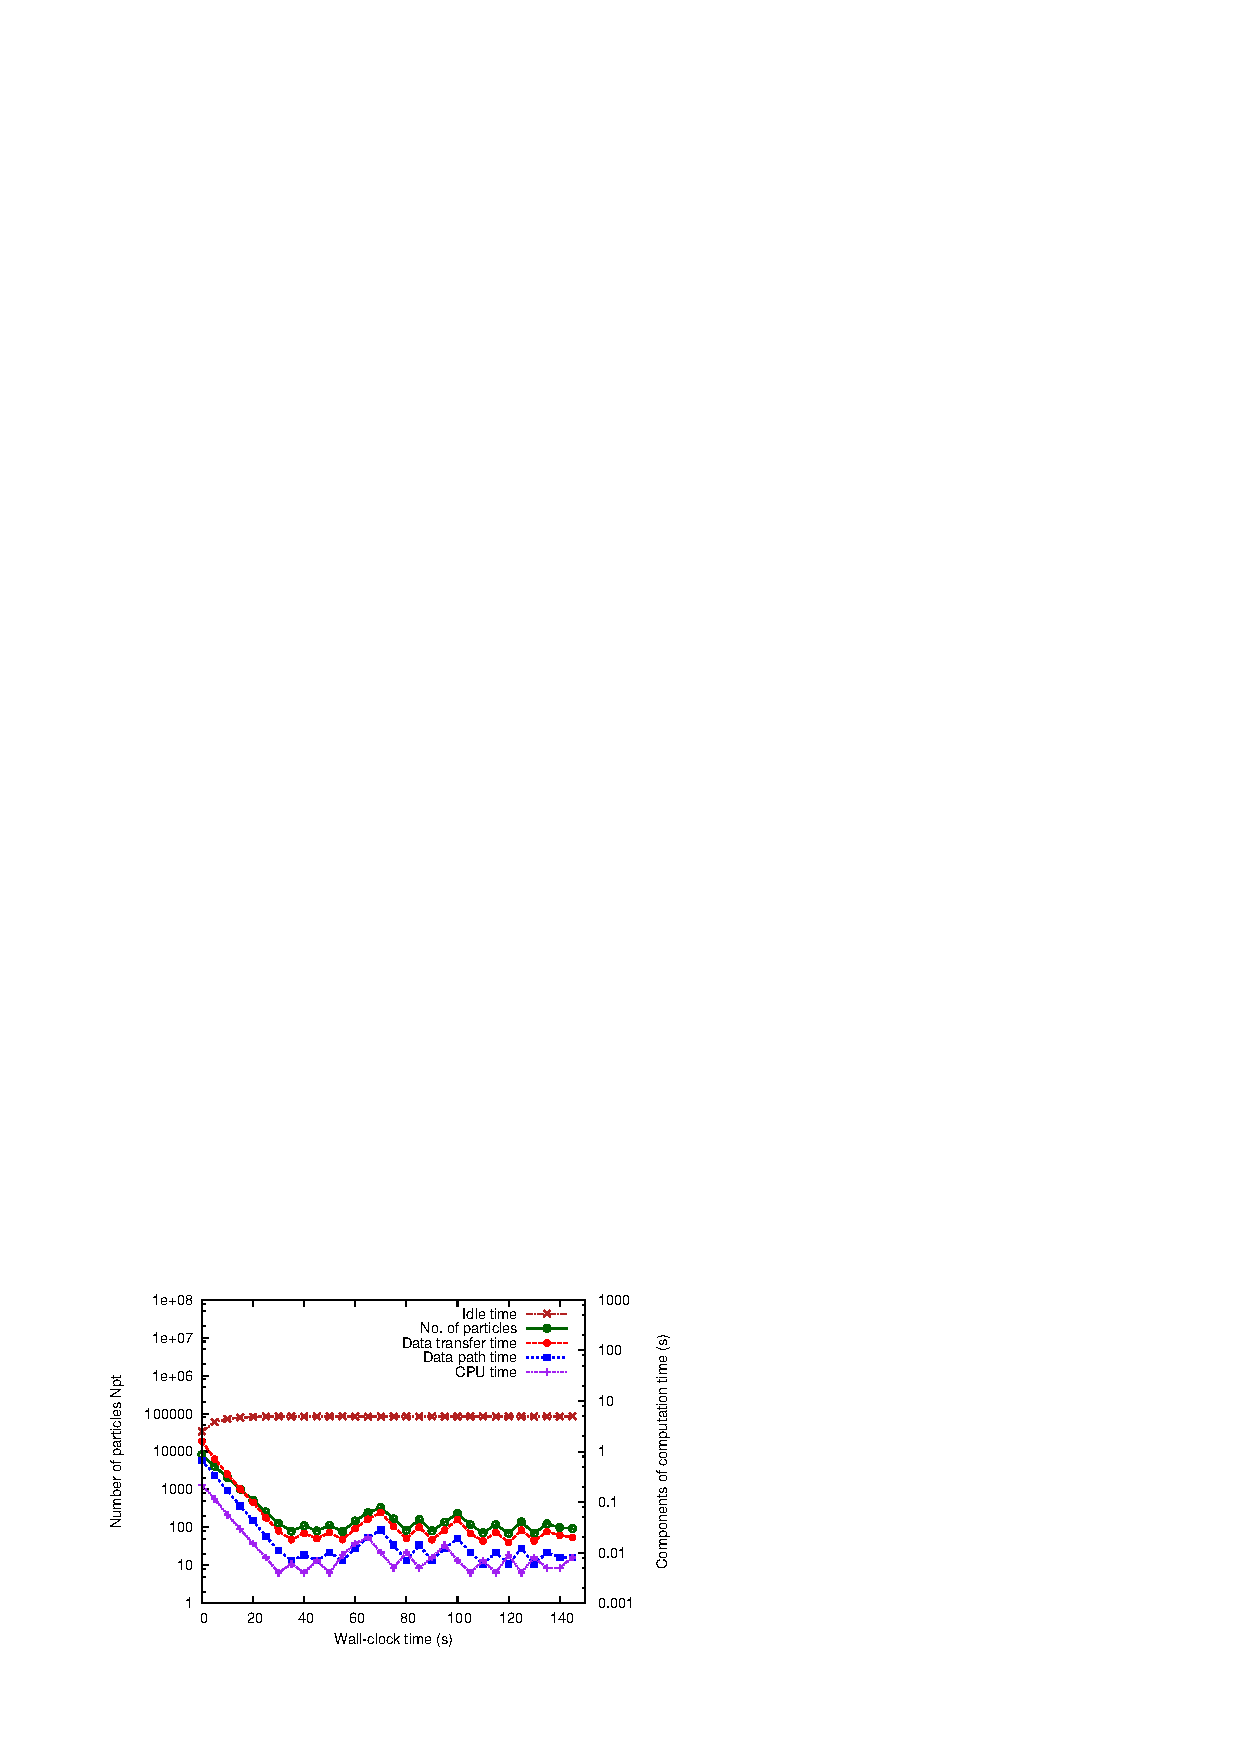
\includegraphics[width=0.7\textwidth]{4_adaptation/figures/fig_adaptive}
\caption{Number of particles and components of total computation time versus wall-clock time.}
\label{fig:adaptive}
\end{figure}

\begin{figure}[t!]
\centering
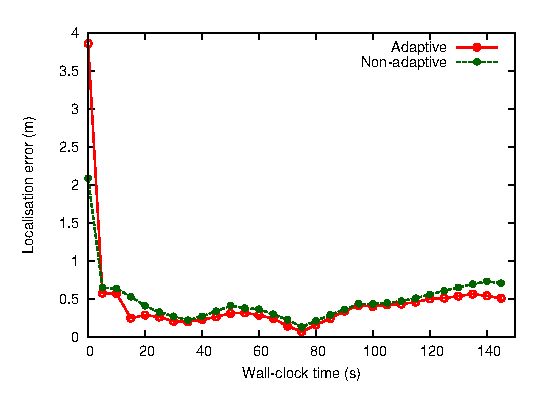
\includegraphics[width=0.7\textwidth]{4_adaptation/figures/fig_error}
\caption{Localisation error versus wall-clock time.}
\label{fig:error}
\end{figure}

\subsection{Data Compression}
Figure~\ref{fig:compression} shows the reduction in data transfer time after applying data compression.
A higher number of replications means a lower data transfer time.
The data transfer time has a lower bound of 0.212 seconds because the data from the \glspl{fpga} to the \glspl{cpu} are not compressible.
Only the particle stream after the resampling process is compressed when it is transferred from the \glspl{cpu} to the \glspl{fpga}.

\begin{figure}[t!]
\centering
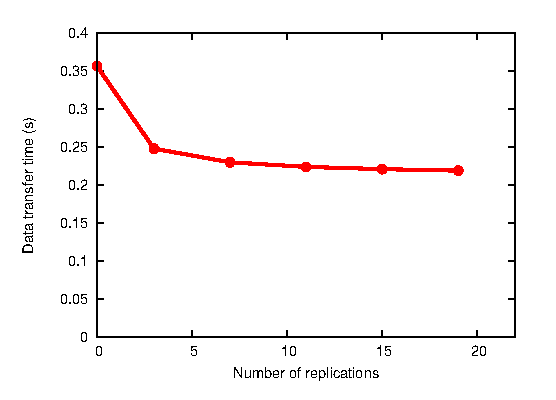
\includegraphics[width=0.7\textwidth]{4_adaptation/figures/fig_compression}
\caption{Effect on the data transfer time by particle stream compression.}
\label{fig:compression}
\end{figure}

\subsection{Performance Comparison of Reconfigurable System, CPU and GPU}
Table~\ref{tab:perf} shows the performance comparison of the \glspl{cpu}, \gls{gpu}s and reconfigurable system.

\textbf{Data-path time}: Considering the time spent on the data-paths only, the reconfigurable system is up to 328 times faster than a single-core \gls{cpu} and 76 times faster than a 12-core \gls{cpu} system with 24 threads.
In addition, it is 12 times and 3 times faster than one \gls{gpu} and four \gls{gpu}s, respectively.

\textbf{Data transfer time}: The data transfer time of reconfigurable system is shown in three rows.
The first row shows the situation when the PCI Express bandwidth is 2 GB/s.
The second row shows the performance when PCI Express gen3 x8 (7.88 GB/s) is used such that the bandwidth is comparable with that of the \gls{gpu} system.
When multiple \gls{fpga} boards are used, the data transfer time decreases because multiple PCI Express buses are utilised simultaneously.
The third row shows the performance when data compression is applied and it is assumed that each particle is replicated for 20 times in average.

\textbf{\gls{cpu} time}: The \gls{cpu} time of reconfigurable system is shorter than that of the \gls{cpu} and \gls{gpu} systems because part of the resampling process of object-particles is performed on the \gls{fpga} using \gls{imh} resampling algorithm~\cite{miao11}.
\gls{imh} resampling algorithm is optimised for the deep pipeline architecture where each particle occupies a single stage of the pipeline.
On the \glspl{cpu} and \gls{gpu}, the computation of the particles are shared by threads and therefore \gls{imh} resampling algorithm is not applicable.

\textbf{Total computation time}: Considering the overall system performance, reconfigurable system is up to 169 times faster than a single-core \gls{cpu}, 41 times faster than a 12-core \gls{cpu} system.
In addition, it is 9 times faster than one \gls{gpu}, and 3 times faster than four \gls{gpu}s.
Notice that the \glspl{cpu} violate the real-time constraint of 5 seconds.

%\newcolumntype{g}{>{\columncolor{Gray}}c}
\begin{table}[ht]
\label{tab:comparison}
\footnotesize
\setlength{\tabcolsep}{1pt}
\begin{spacing}{1.0}
\caption{Performance comparison of reconfigurable system (RS), CPU and GPU.}
\label{tab:perf}
	\centering
		\smallskip
		\begin{threeparttable}
		\begin{tabular}{l || c c c c c g g g}
		\hline
												& \gls{cpu}(1) $^a$ 					& \gls{cpu}(2) $^a$ 				& \gls{gpu}(1) $^b$ 				& \gls{gpu}(2) $^b$ 				& \gls{gpu}(3) $^b$ 				& RS(1) $^c$& RS(2) $^d$& RS(3) $^d$ \\
		\hline
		\hline
		Clock frequency (MHz) 						& 2660							& 2660 						& 1150  					& 1150						& 1150						& 100  		&  100 		& 100 		\\
		\multirow{2}{*}{Precision}				& \multirow{2}{*}{single}		& \multirow{2}{*}{single} 	& \multirow{2}{*}{single} 	& \multirow{2}{*}{single} 	& \multirow{2}{*}{single} 	& single	& single	& single	\\
												&								&							&							&							&							& + custom	& + custom	& + custom	\\
		Level of parallelism					& 1								& 24						& 448   					& 896						& 1792						& 2+8 $^e$ 	& 4+24 $^e$ & 8+24 $^e$ \\
		\hline
		Data-path time (s) 		   				& 27.530							& 6.363 					& 1.000						& 0.500						& 0.250						& 0.336 	& 0.168 	& 0.084 	\\
		Data-path speedup						& 1x							& 4.3x 						& 27.5x 					& 55.1x						& 110.1x					& 81.9x 	& 163.9x	& 327.7x 	\\
		\multirow{3}{*}{Data transfer time (s)} 	& \multirow{3}{*}{0}			& \multirow{3}{*}{0}		& \multirow{3}{*}{0.360} 	& \multirow{3}{*}{0.180} 	& \multirow{3}{*}{0.090} 	& 1.432 $^f$& 0.716 $^f$& 0.358 $^f$\\
												&								& 							& 							& 							&							& 0.363 $^g$& 0.182 $^g$& 0.091 $^g$\\
												&								& 							& 							& 							&							& 0.223 $^h$& 0.111 $^h$& 0.056 $^h$\\
		\gls{cpu} time (s)							& 0.420							& 0.334						& 0.117						& 0.117						& 0.117						& 0.030		& 0.025		& 0.025		\\
		Total comp. time (s)  					& 27.95							& 6.697 					& 1.477						& 0.797						& 0.457						& 0.589 	& 0.304		& 0.165 	\\
		Overall speedup  						& 1x							& 4.2x	 					& 18.9x						& 35.1x						& 61.2x						& 47.5x 	& 91.9x		& 169.4x	\\
		\hline
		Computation power (W) 	   					& 183							& 279 						& 287  						& 424						& 698						& 145 		& 420		& 480		\\
		Computation power eff.						& 1x							& 0.7x						& 0.6x 						& 0.4x						& 0.3x						& 1.3x 		& 0.4x 		& 0.4x		\\
		Idle power (W)    						& 133							& 133						& 208   					& 266 						& 382						& 95		& 360		& 360		\\
		Idle power eff.					    	& 1x							& 1x						& 0.6x	 					& 0.5x						& 0.4x						& 1.4x 	& 0.4x		& 0.4x		\\
		\hline
		Energy. (J) $^i$						& 677/5115						& 673/1868 					& 1041/1157 				& 1331/1456					& 1911/2054					& 489/595 	& 1896/1914	& 1994/2012	\\
		Energy eff.							& 1x							& 1x/2.7x 					& 0.7x/4.4x 				& 0.5x/3.5x 				& 0.4x/2.5x					& 1.4x/8.6x	& 0.4x/2.7x	& 0.3x/2.5x\\
		\hline
		\end{tabular}
			\begin{tablenotes}
			\item[a] 2 Intel Xeon X5650 \glspl{cpu} @2.66 GHz (12 cores supporting 24 threads).
			\item[b] 1/2/4 NVIDIA Tesla C2070 \gls{gpu}s and 1 Intel Core i7-950 \gls{cpu} @3.07 GHz (4 cores supporting 8 threads).
			\item[c] 1 Xilinx XC6VSX475T \gls{fpga} and 1 Intel Core i7-870 \gls{cpu} @2.93 GHz (4 cores supporting 8 threads).
			\item[d] 4 Xilinx XC6VSX475T \glspl{fpga} and 2 Intel Xeon X5650 \glspl{cpu} @2.66 GHz (12 cores supporting 24 threads).
			\item[e] Number of \gls{fpga} data-paths and number of \gls{cpu} threads.
			\item[f] Each \gls{fpga} communicates with \glspl{cpu} via a PCI Express bus with 2 GB/s bandwidth.
			\item[g] Each \gls{fpga} communicates with \glspl{cpu} via a PCI Express Gen3 x8 bus with 7.88 GB/s bandwidth.
			\item[h] Each \gls{fpga} communicates with \glspl{cpu} via a PCI Express Gen3 x8 bus with data compression.
			\item[i] Cases for 573k and 67M particles in a 5-second interval.
			\end{tablenotes}
		\end{threeparttable}
\end{spacing}
\end{table}

\textbf{Power and energy consumption}: In real-time applications, we are interested in the energy consumption per time-step.
Figure~\ref{fig:power} shows the power consumption of reconfigurable system, \glspl{cpu} and \gls{gpu} over a period of 10 seconds (two time-steps).
The system power is measured using a power meter which is connected directly between the power source and the system.
All the curves of reconfigurable system show peaks when the system is at the computation mode and troughs when it is at the low power mode.
The power during the configuration period lies between the two modes.
On the reconfigurable system with one \gls{fpga}, run-time reconfiguration reduces the idle power consumption by 34\% from 145W to 95W.
In other words, over a 5-second time-step, the energy consumption is reduced by up to 33\%.
On the reconfigurable system with four \glspl{fpga}, the idle power consumption is reduced by 25\% from 480W to 360W, and hence the energy consumption decreased by up to 17\%.

The run-time reconfiguration methodology is not limited to the Maxeler systems, it can be applied to other \gls{fpga} platforms.
The resource management software of our system (MaxelerOS) simplifies the effort of performing run-time reconfiguration, and hence we can focus on studying the impact of run-time reconfiguration on energy saving.

\begin{figure}[t!]
\centering
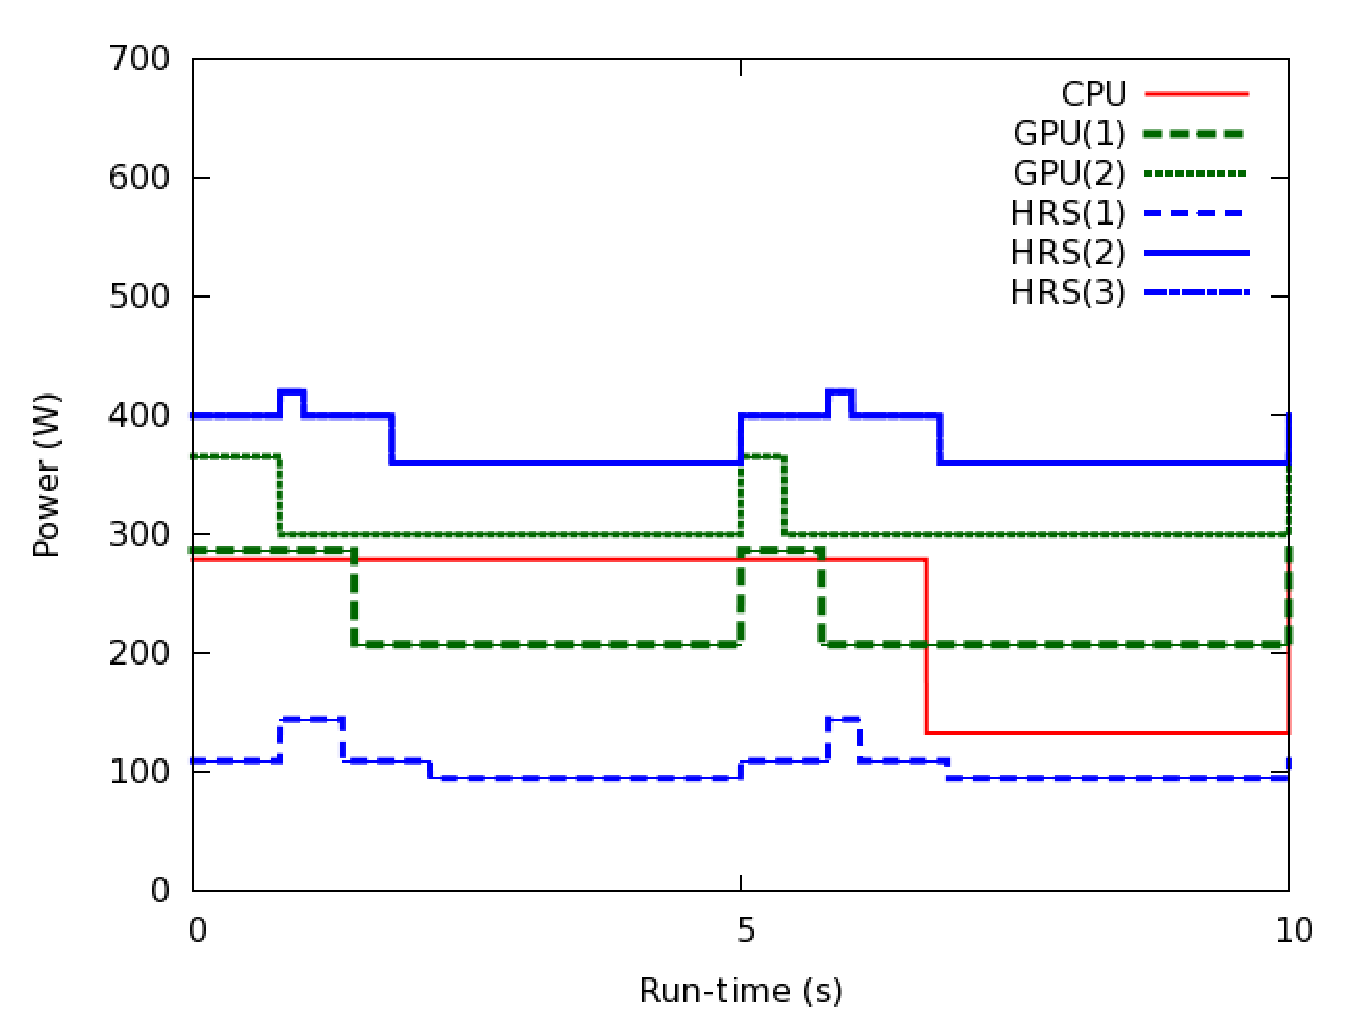
\includegraphics[width=0.8\textwidth]{4_adaptation/figures/fig_power2}
\caption[Power consumption of reconfigurable system (RS), CPU and GPU in one time-step, notice that the computation time of the CPU system exceeds the 5-second real-time requirement]{Power consumption of reconfigurable system (RS), CPU and GPU in one time-step, notice that the computation time of the CPU system exceeds the 5-second real-time requirement (The lines of RS(2) and RS(3) overlap).}
\label{fig:power}
\end{figure}

To identify the speed and energy trade-off, we produce a graph as shown in Figure~\ref{fig:scale}. 
Each data point represents the computation time versus energy consumption of a system setting.
Among all the systems, the reconfigurable system with one \gls{fpga} has the computation speed satisfying the real-time requirement, while consuming the smallest amount of energy.
All the configurations of \gls{cpu} system cannot meet the real-time requirement.
RS(3), the reconfigurable system with four \glspl{fpga}, is the fastest among all the systems in comparison, therefore it is able to handle larger problems and more complex applications.

\begin{figure}[t!]
\centering
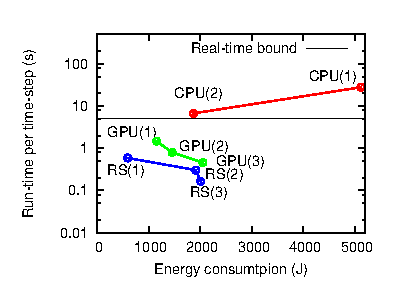
\includegraphics[width=0.7\textwidth]{4_adaptation/figures/fig_scale}
\caption[Run-time versus energy consumption of reconfigurable system (RS), CPU and GPU]{Run-time versus energy consumption of reconfigurable system (RS), CPU and GPU (5-second time-step, 67M particles; Refer to Table~II for system settings).}
\label{fig:scale}
\end{figure}


%%%%%%%%%%%%%%%%%%%%%%%%%%%%%%%%%%%%%%%%
\section{Summary}
\label{sec:reconfig_summary}

This chapter presents an approach for accelerating adaptive particle filter for real-time applications.
The proposed heterogeneous reconfigurable system demonstrates a significant reduction in power and energy consumption compared with \gls{cpu} and \gls{gpu}.
The adaptive algorithm reduces computation time while maintaining the quality of results. 
The approach is scalable to systems with multiple \glspl{fpga}.
A data compression technique is used to mitigate the data transfer overhead between the \glspl{fpga} and \glspl{cpu}.


%%%%%%%%%%%%%%%%%%%%%%%%%%%%%%%%%%%%%%%%

